\documentclass{article}
\usepackage{tikz}
\usetikzlibrary{shapes,arrows,automata, positioning, arrows}
\begin{document}
\pagestyle{empty}


% Define block styles
\tikzstyle{decision} = [diamond, draw, fill=blue!20, 
text width=4.5em, text badly centered, node distance=3cm, inner sep=0pt]
\tikzstyle{block} = [rectangle, draw, fill=blue!20, 
text width=5em, text centered, rounded corners, minimum height=4em]
\tikzstyle{line} = [draw, -latex']
\tikzstyle{cloud} = [draw, ellipse,fill=red!20, node distance=3cm,
minimum height=2em]

\begin{tikzpicture}[node distance = 2cm, auto]
	% Place nodes
	\node [block] (init) {initialize model};
	\node [cloud, left of=init] (expert) {expert};
	\node [cloud, right of=init] (system) {system};
	\node [block, below of=init] (identify) {identify candidate models};
	\node [block, below of=identify] (evaluate) {evaluate candidate models};
	\node [block, left of=evaluate, node distance=3cm] (update) {update model};
	\node [decision, below of=evaluate] (decide) {is best candidate better?};
	\node [block, below of=decide, node distance=3cm] (stop) {stop};
	% Draw edges
	\path [line] (init) -- (identify);
	\path [line] (identify) -- (evaluate);
	\path [line] (evaluate) -- (decide);
	\path [line] (decide) -| node [near start] {yes} (update);
	\path [line] (update) |- (identify);
	\path [line] (decide) -- node {no}(stop);
	\path [line,dashed] (expert) -- (init);
	\path [line,dashed] (system) -- (init);
	\path [line,dashed] (system) |- (evaluate);
\end{tikzpicture}

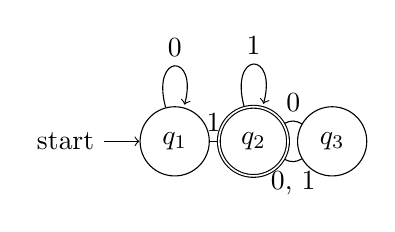
\begin{tikzpicture}
	\node[state, initial] (q1) {$q_1$};
	\node[state, accepting, right of=q1] (q2) {$q_2$};
	\node[state, right of=q2] (q3) {$q_3$};
	\draw (q1) edge[loop above] node{0} (q1)
	(q1) edge[above] node{1} (q2)
	(q2) edge[loop above] node{1} (q2)
	(q2) edge[bend left, above] node{0} (q3)
	(q3) edge[bend left, below] node{0, 1} (q2);
\end{tikzpicture}

\end{document}
